\section{A uniform estimate for an annular twist}\label{sec:annulus}

We apply the fourth-variation estimate to an annulus with two prescribed
boundary directions.  The aim is to bound uniformly how much its partition
function changes when one boundary direction rotates.  The spatial tests
will be defined on the full annulus and then restricted to the retained
graph.
In this section, $C$ denotes a finite constant depending only on the
fixed smooth profiles, and $C_\beta$ may also depend on $\beta$;
these constants may increase from one estimate to the next.

For an integer $N\geq 2$, let
\[
 D_N=\{x\in\Z^2:N\leq\|x\|_\infty\leq 2N\}.
\]
Let $G=(V,E)$ be any subgraph of the nearest-neighbor graph on $D_N$,
and orient each edge in a positive coordinate direction.  Give its edges
strengths $0\leq b_e\leq\beta$.  Put $s_*=(1,0,0)$ and prescribe
\[
 s_x=\exp(tc)s_*\quad(\|x\|_\infty=N),
 \qquad
 s_x=s_*\quad(\|x\|_\infty=2N)
 \quad (x\in V).
\]
All other spins are integrated against uniform probability measure on
$S^2$.  Write $Z(t)$ for the resulting partition integral, including the
interactions between any prescribed spins.  Missing vertices on either
boundary require no additional convention: only vertices of $V$ are
pinned.

\begin{proposition}[Vanishing annular twist cost]\label{prop:annulus}
For every finite $\beta>0$ there is a finite constant $C_\beta$ such that,
for all $N\geq2$ and all graphs and strengths just described,
\begin{equation}\label{eq:annulus-minmax}
 \frac{\min_{t\in\R}Z(t)}{\max_{t\in\R}Z(t)}
 \geq 1-\frac{C_\beta}{\log N}.
\end{equation}
In particular,
\begin{equation}\label{eq:annulus-ratio}
 \frac{Z(\pi)}{Z(0)}\geq1-\frac{C_\beta}{\log N}.
\end{equation}
The constant is independent of the subgraph, the strength array, and
the twist parameter.
\end{proposition}

\subsection{Boundary gauge and multiscale tests}

Fix once and for all a real smooth function $\Theta$ equal to one in a
neighborhood of $[-1,1]^2$ and compactly supported in $(-2,2)^2$.  Define
the real edge form
\begin{equation}\label{eq:annulus-h}
 h_e=\Theta(y/N)-\Theta(x/N),\qquad e=(x,y).
\end{equation}
Use a subscript $t$ on $W,X,H_k,R$ for the quantities from the preceding
section evaluated with these boundary values, and write
$\langle\,\cdot\,\rangle_t$ for the corresponding expectation.  Although
$\Theta$ does not vanish on the inner pinned layer, its gauge action is
still explicit:
\begin{equation}\label{eq:annulus-boundary-gauge}
 W_t(shc)=\frac{Z(t+s)}{Z(t)},
 \qquad
 R_t(h,h)=-\frac{Z''(t)}{Z(t)}.
\end{equation}
Indeed, substituting
$s_x^{\mathrm{old}}=\exp(-s\Theta(x/N)c)s_x^{\mathrm{new}}$
cancels every edge matrix.  It changes the inner boundary value to
$\exp((t+s)c)s_*$ and leaves the outer value unchanged.  Thus the gauge
changes the prescribed boundary values, rather than treating them as
integrated variables.

The analytic target is now an upper bound of order $1/\log N$ for
$R_t(h,h)$.  We will construct functions whose collective form
$\sum_i S(f_i,\overline{f_i})$ equals $-i\lambda_N\widetilde h$,
where $\lambda_N\geq\tfrac12\log N$ and $\widetilde h$ approximates $h$.
The two family costs in Proposition~\ref{prop:fourth} will total
$O(\log N)$, whereas bilinearity multiplies
$R_t(\widetilde h,\widetilde h)$ by $\lambda_N^2$.
This yields the required logarithmic gain; after constructing the family,
we will transfer the bound from $\widetilde h$ to $h$ without assuming
that $R_t$ is positive.

For $m=1,2$, put $g_m=\partial_m\Theta$.  Choose a real smooth cutoff
$\chi_m$ compactly supported in
\[
 \mathcal A=\{z\in\R^2:1<\|z\|_\infty<2\}
\]
and equal to one on $\operatorname{supp}g_m$.  Such a cutoff exists
because $g_m$ vanishes near both boundary squares.  The real profiles
\begin{equation}\label{eq:annulus-profiles}
 \phi_{m,+}=\frac{\chi_m+g_m}{2},\qquad
 \phi_{m,-}=\frac{\chi_m-g_m}{2}
 \quad\hbox{satisfy}\quad
 \phi_{m,+}^2-\phi_{m,-}^2=g_m.
\end{equation}
This construction uses no square root of a signed smooth function.
All four profiles have compact support in $\mathcal A$.
Figure~\ref{fig:annulus-tests} shows how these supports lie between
the two pinned layers.

\begin{figure}[htbp]
\centering
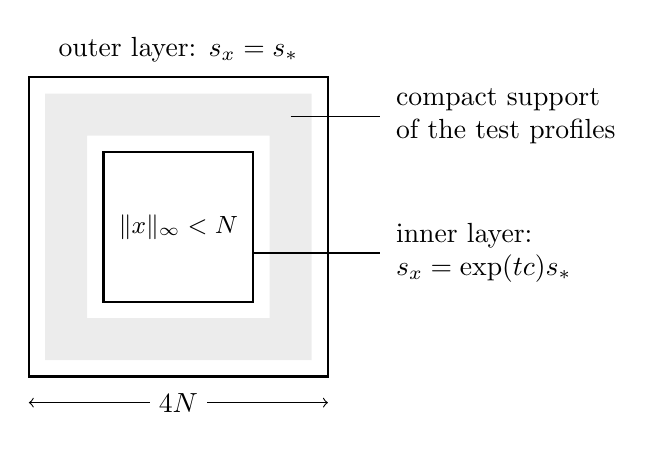
\begin{tikzpicture}[scale=0.95]
 \path[fill=gray!15,even odd rule]
   (-1.78,-1.78) rectangle (1.78,1.78)
   (-1.22,-1.22) rectangle (1.22,1.22);
 \draw[thick] (-2,-2) rectangle (2,2);
 \draw[thick] (-1,-1) rectangle (1,1);
 \node[font=\small] at (0,0) {$\|x\|_\infty<N$};
 \node[anchor=south] at (0,2.08)
   {outer layer: $s_x=s_*$};
 \draw (1,-0.35) -- (2.7,-0.35);
 \node[anchor=west,align=left] at (2.78,-0.35)
   {inner layer:\\$s_x=\exp(tc)s_*$};
 \draw (1.5,1.48) -- (2.7,1.48);
 \node[anchor=west,align=left] at (2.78,1.48)
   {compact support\\of the test profiles};
 \draw[<->] (-2,-2.35) -- (2,-2.35);
 \node[fill=white] at (0,-2.35) {$4N$};
\end{tikzpicture}
\caption{The boundary twist is tested using profiles supported strictly
between the pinned squares.  The shaded region is schematic: one fixed
compact subannulus contains all four profile supports.  The estimates
remain valid when arbitrary vertices and edges are deleted.}
\label{fig:annulus-tests}
\end{figure}

For $p\in\Z^2$ let $r_p=\|p\|_\infty$.  Introduce four groups of
vertex functions, restricted to $V$:
\begin{equation}\label{eq:annulus-modes}
 f_{m,\pm,p}(x)
 =r_p^{-3/2}\phi_{m,\pm}(x/N)
       \exp\left(\frac{2\pi i\,p\cdot x}{16N}\right),
 \qquad
 1\leq r_p\leq N,\quad \pm p_m>0.
\end{equation}
They vanish at every pinned vertex.  The power $r_p^{-3/2}$ is chosen
to produce a harmonic sum: the shell face $p_m=\pm r$ contains $2r+1$ modes, each with
squared normalization $r^{-3}$ and coordinate-$m$ phase increment of order
$r/N$.  Its summed frequency factor in the commutator is therefore of
order $1/(Nr)$.  The opposite frequency signs give the adjacent-point
products of $\phi_{m,+}$ and $\phi_{m,-}$ opposite coefficients.
Index this finite family by $i$, write $u_i=df_i$, and, as in
Proposition~\ref{prop:fourth}, put
\[
 T_{e\ell}=\sum_i u_i(e)\overline{u_i(\ell)},
 \qquad
 S(f,g)_e=\tfrac12(f_xg_y-g_xf_y).
\]
For an edge $e=(x,x+e_m)$ define
\begin{equation}\label{eq:annulus-htilde}
 \widetilde h_e=\frac1N
 \left[
 \phi_{m,+}(x/N)\phi_{m,+}((x+e_m)/N)
 -\phi_{m,-}(x/N)\phi_{m,-}((x+e_m)/N)
 \right].
\end{equation}

\begin{lemma}[The multiscale family]\label{lem:modes}
There is a constant $C$, depending only on the fixed profiles, with the
following properties for every $N\geq2$ and every such subgraph.
First,
\begin{equation}\label{eq:annulus-commutator}
 \sum_i S(f_i,\overline{f_i})=-i\lambda_N\widetilde h,
 \qquad
 \lambda_N
 =N\!\!\sum_{\substack{1\leq r_p\leq N\\p_1>0}}
      r_p^{-3}\sin\left(\frac{2\pi p_1}{16N}\right)
 \geq\frac12\sum_{r=1}^N\frac1r.
\end{equation}
Second,
\begin{equation}\label{eq:annulus-midpoint}
 \|h\|_2\leq C,\qquad
 \|h+\widetilde h\|_\infty\leq\frac CN,\qquad
 \|h-\widetilde h\|_1\leq\frac CN.
\end{equation}
Finally,
\begin{equation}\label{eq:annulus-test-cost}
 \|T\|_{\mathrm{HS}}^2+
 \sum_{i,j}\min\left\{
   \|f_i\|_\infty^2\|df_j\|_2^2,
   \|f_j\|_\infty^2\|df_i\|_2^2
 \right\}
 \leq C(1+\log N).
\end{equation}
All edge norms use counting measure on $E$.
\end{lemma}

\begin{proof}
For a real profile $\phi$ and one mode on shell $r_p$, direct substitution
on a positive coordinate-$j$ edge gives
\begin{equation}\label{eq:annulus-one-mode}
 S(f_p,\overline{f_p})_e
 =-i r_p^{-3}\phi(x/N)\phi((x+e_j)/N)
       \sin\left(\frac{2\pi p_j}{16N}\right).
\end{equation}
If the group is indexed by $m\ne j$, its frequency set is invariant
under $p_j\mapsto-p_j$, so its sum vanishes.  For $m=j$, the negative
half-plane gives the negative of the positive-half-plane sine sum.
Interchanging coordinates identifies the positive sums for $j=1,2$.
This proves the identity in \eqref{eq:annulus-commutator}.

On shell $r$, retain only the $2r+1$ frequencies with $p_1=r$ and
$|p_2|\leq r$.  Since
\[
 \sin\left(\frac{\pi r}{8N}\right)\geq\frac r{4N}
 \qquad(1\leq r\leq N),
\]
their contribution to $\lambda_N$ is at least
$(2r+1)/(4r^2)\geq1/(2r)$.  This gives its asserted lower bound.

For an edge in direction $m$, let $z=(x+y)/(2N)$.  Centered Taylor
expansion, with uniform bounds on the fixed smooth functions, gives
\[
 h_e=N^{-1}\partial_m\Theta(z)+O(N^{-3}),\qquad
 \phi(x/N)\phi(y/N)=\phi(z)^2+O(N^{-2}).
\]
Using \eqref{eq:annulus-profiles} yields
$|h_e-\widetilde h_e|\leq C N^{-3}$.  There are $O(N^2)$ annulus
edges, and $|h_e|+|\widetilde h_e|\leq C/N$.  The three estimates in
\eqref{eq:annulus-midpoint} follow, also after restriction to $E$.

For a mode on shell $r$, the product rule for a discrete difference
and $|e^{iv}-1|\leq|v|$ give
\begin{equation}\label{eq:annulus-mode-norms}
 \|f_i\|_\infty\leq Cr^{-3/2},\qquad
 \|df_i\|_2\leq Cr^{-3/2}(1+r)\leq C' r^{-1/2}.
\end{equation}
There are $O(r)$ modes on shell $r$, including all four groups.
For shells $s\leq r$, choose the bound in the minimum that uses the
supremum norm of the shell-$r$ mode.  The cost of a pair is at most
$Cr^{-3}s^{-1}$; all $O(rs)$ pairs therefore cost at most $Cr^{-2}$.
Summing both shell orderings gives
\begin{equation}\label{eq:annulus-minimum-sum}
 \sum_{i,j}\min\left\{
   \|f_i\|_\infty^2\|df_j\|_2^2,
   \|f_j\|_\infty^2\|df_i\|_2^2
 \right\}
 \leq C\sum_{r=1}^N\sum_{s=1}^r r^{-2}
 \leq C'(1+\log N).
\end{equation}

It remains to bound $T$.  Applying the triangle inequality mode by mode
would give only $\|T\|_{\mathrm{HS}}\leq\sum_i\|df_i\|_2^2=O(N)$;
we use Fourier orthogonality for the sharper bound.  Work first in a
single profile group and let $U$ be the matrix whose $p$-th column is
$r_p^{1/2}df_p$.
Embed the annulus in the discrete torus
$Q_N=(\Z/(16N)\Z)^2$.  Its representatives may be chosen in
$[-8N,8N-1]^2$; all profiles vanish near the boundary of this square,
so they also define torus functions.  Let $F$ have columns
\[
 F_{x,p}=\exp\left(\frac{2\pi i\,p\cdot x}{16N}\right),
 \qquad x\in Q_N,
\]
using the frequencies of this group.  They are distinct modulo $16N$,
and orthogonality of these unnormalized waves gives
\begin{equation}\label{eq:annulus-fourier-norm}
 F^*F=(16N)^2I,\qquad \|F\|_{\mathrm{op}}=16N.
\end{equation}
For direction $j$, let $P_j$ restrict functions on $Q_N$ to the
origins of the coordinate-$j$ edges in $E$.  Let $M_v$ denote
multiplication by $v$ on $Q_N$, and set
\[
 \Delta_j\phi(x)=\phi((x+e_j)/N)-\phi(x/N),
 \qquad \phi^{(j)}(x)=\phi((x+e_j)/N).
\]
The directional block of $U$ has the exact factorization
\begin{align}\label{eq:annulus-operator-factorization}
 U_j={}&P_jM_{\Delta_j\phi}F
              \operatorname{diag}(r_p^{-1})\notag\\
 &+P_jM_{\phi^{(j)}}F
   \operatorname{diag}\left(
      \frac{\exp(2\pi i p_j/(16N))-1}{r_p}\right).
\end{align}
Here $\|P_j\|_{\mathrm{op}}\leq1$,
$\|\Delta_j\phi\|_\infty\leq C/N$, and the last diagonal factor
has operator norm at most $C/N$, since $|p_j|\leq r_p$.
Equation~\eqref{eq:annulus-fourier-norm} now gives
$\|U_j\|_{\mathrm{op}}\leq C$ and hence
$\|U\|_{\mathrm{op}}\leq C$ after combining the two directions.

The contribution of this group is
\[
 T_{\mathrm{group}}=U\operatorname{diag}(r_p^{-1})U^*.
\]
The finite-matrix inequality
$\|ADB\|_{\mathrm{HS}}\leq
\|A\|_{\mathrm{op}}\|D\|_{\mathrm{HS}}\|B\|_{\mathrm{op}}$
therefore implies
\[
 \|T_{\mathrm{group}}\|_{\mathrm{HS}}^2
 \leq C\sum_p r_p^{-2}
 \leq C'\sum_{r=1}^N r\,r^{-2}
 \leq C''(1+\log N).
\]
The triangle inequality over the four groups gives the same order
for $\|T\|_{\mathrm{HS}}^2$.  Together with
\eqref{eq:annulus-minimum-sum}, this proves
\eqref{eq:annulus-test-cost}.
\end{proof}

\subsection{From the test form to the boundary twist}

\begin{proof}[Proof of Proposition~\ref{prop:annulus}]
Apply Proposition~\ref{prop:fourth} in the law with twist $t$, using
the family \eqref{eq:annulus-modes}.  The left side is
\[
 R_t(-i\lambda_N\widetilde h,i\lambda_N\widetilde h)
 =\lambda_N^2R_t(\widetilde h,\widetilde h),
\]
because $R_t$ is bilinear and $\widetilde h$ is real.
Lemma~\ref{lem:modes} gives, uniformly in $t$,
\begin{equation}\label{eq:annulus-tested-response}
 R_t(\widetilde h,\widetilde h)
 \leq\frac{C_\beta(1+\log N)}{(\log N)^2}
 \leq\frac{C'_\beta}{\log N}.
\end{equation}

We must transfer this upper bound to $h$ without treating $R_t$ as a
positive form.  If $R_t(h,h)\leq0$, the desired positive upper bound
already holds.  Otherwise, the defining second-derivative identity
and the pointwise bound on $H_{2,t}$ give
\begin{equation}\label{eq:annulus-current-control}
 \langle X_t(hc)^2\rangle_t
 <-\langle H_{2,t}(hc,hc)\rangle_t
 \leq\beta\|h\|_2^2\leq C\beta.
\end{equation}
Put $d=h-\widetilde h$.  The current is a real random variable on
real edge forms, and
\[
 |X_t(dc)|\leq\beta\|d\|_1\leq\frac{C\beta}{N}.
\]
Consequently ordinary Cauchy--Schwarz for random variables, followed
by \eqref{eq:annulus-current-control}, yields
\begin{align}\label{eq:annulus-current-error}
 \left|\langle X_t(hc)^2-X_t(\widetilde h c)^2\rangle_t\right|
 &\leq
 2\langle X_t(hc)^2\rangle_t^{1/2}
       \|X_t(dc)\|_\infty+\|X_t(dc)\|_\infty^2\notag\\
 &\leq\frac{C_\beta}{N}.
\end{align}
The local quadratic term satisfies the stronger pointwise bound
\begin{align}\label{eq:annulus-local-error}
 |H_{2,t}(hc,hc)-H_{2,t}(\widetilde h c,\widetilde h c)|
 &\leq\beta\sum_{e\in E}|d_e|\,|h_e+\widetilde h_e|\notag\\
 &\leq\frac{C\beta}{N^2}.
\end{align}
Equations~\eqref{eq:annulus-tested-response}--\eqref{eq:annulus-local-error}
and the formula for $R_t$ imply in both cases that
\begin{equation}\label{eq:annulus-ode}
 -\frac{Z''(t)}{Z(t)}=R_t(h,h)
 \leq\frac{C_\beta}{\log N}+\frac{C_\beta}{N}
 \leq\delta_N,\qquad
 \delta_N=\frac{C'_\beta}{\log N}.
\end{equation}
All constants are independent of the boundary twist, the retained
vertices and edges, and the admissible strengths.

Finally, $Z$ is positive, smooth, and $2\pi$-periodic.  Set
$M=\max_t Z(t)$ and choose $t_0$ with $Z(t_0)=M$.  Then
$Z'(t_0)=0$, and \eqref{eq:annulus-ode} implies
$Z''(t)\geq-\delta_N Z(t)\geq-\delta_N M$.
For any $t$, choose an orientation $\epsilon\in\{-1,1\}$ and
$0\leq\ell\leq\pi$ with $t=t_0+\epsilon\ell$ modulo $2\pi$.
Twice integrating the second-derivative bound for
$v\mapsto Z(t_0+\epsilon v)$ gives
\[
 Z(t)\geq M-\frac{\delta_N M\ell^2}{2}
 \geq M\left(1-\frac{\pi^2\delta_N}{2}\right).
\]
Taking the minimum and enlarging $C_\beta$ proves
\eqref{eq:annulus-minmax}.  Since
$Z(\pi)/Z(0)\geq\min Z/\max Z$, it also proves
\eqref{eq:annulus-ratio}.
\end{proof}
